\documentclass[10pt,landscape,a4paper]{article}
\usepackage[utf8]{inputenc}
\usepackage[english]{babel}
\usepackage[utopia,sfscaled]{mathdesign}
\usepackage{multicol}
\usepackage[top=2mm,bottom=2mm,left=1mm,right=1mm]{geometry}
\usepackage{lipsum}
\usepackage{microtype}
\usepackage{graphicx}
\usepackage{amsmath}
\usepackage{breqn}
\usepackage{enumitem}
\usepackage{titlesec}

\setitemize{noitemsep,topsep=0pt,parsep=0pt,partopsep=0pt}
\setenumerate{noitemsep,topsep=0pt,parsep=0pt,partopsep=0pt}
\setlength{\parindent}{0pt}
\setlength{\parskip}{0.2\baselineskip}
\titleformat*{\section}{\footnotesize\bfseries}
\titleformat*{\subsection}{\scriptsize\bfseries}
\titlespacing{\section}{0pt}{\parskip}{-\parskip}
\titlespacing{\subsection}{0pt}{\parskip}{-\parskip}

\newcommand{\N}{\mathbb{N}}
\newcommand{\set}[1]{\left \{ #1 \right \}}
\newcommand{\abs}[1]{\left | #1 \right |}
\newcommand{\ceil}[1]{\left \lceil #1 \right \rceil}
\newcommand{\encoding}[1]{\left \langle #1 \right \rangle}

\graphicspath{{images/}}

\begin{document}
\small

\begin{multicols*}{3}

\section{Regular Languages}

\subsection{Closure Properties}

\begin{itemize}
    \item Union
    \item Concatenation
    \item Star
    \item Intersection: $L_1 \cap L_2 = \overline{\overline{L_1} \cup \overline{L_2}}$
    \item Difference $L_1 \setminus L_2 = L_1 \cap \overline{L_2}$
\end{itemize}

\textbf{Tips}:

\begin{itemize}
    \item If $L_1$ and $L_2$ are bot not regular, is $L_1 \cup L_2$ necessarily not regular? No. Let $L_1$ be not regular (e.g. $\set{0^n, 1^n}$) and $L_2 = \overline{L_1}$. Then $L_1 \cup L_2 = \Sigma^*$ is regular.
\end{itemize}

\subsection{Pumping Lemma}

If $A$ is a regular language, then there is an integer $p$ where $\exists s \in A$ of length at least $p$, then $s = xyz$, satisfying the following conditions:

\begin{itemize}
    \item $\forall i \geq 0, xy^iz \in A$,
    \item $\abs{y} > 0$,
    \item $\abs{xy} \leq p$.
\end{itemize}

\textbf{Tips}:

\begin{itemize}
    \item To prove $L$ is not regular, we can use another regular $L'$ (e.g. $\set{0^n1^m: n, m \in \N}$). Apply Pumping Lemma on $L \cap L'$.
\end{itemize}

\section{Context-Free Languages}

\textbf{Examples}:

\underline{\#$a$'s = \#$b$'s}

$S \rightarrow aSbS | bSaS | \epsilon$

\underline{\#$a$'s $\geq$ \#$b$'s}

$S \rightarrow SS | aSbS | bSaS | a | \epsilon$

\underline{\#$a$'s = 2\#$b$'s}

$S \rightarrow \epsilon | SS | aSaSb | aSbSa | bSaSa$

\subsection{Closure Properties}

\begin{itemize}
    \item Union: $S \rightarrow S_1 | S_2$
    \item Concatenation: $S \rightarrow S_1S_2$
    \item Star: $S \rightarrow SS_1 | \epsilon$
\end{itemize}

\section{Turing Machines}

\subsection{Closure Properties}

Decidable languages are closed under:

\begin{itemize}
    \item Union: $M$ = Run $M_1$ \& $M_2$ at the same time, if either of them accepts, accept; otherwise reject.
    \item Intersection: $M$ = $M$ = Run $M_1$ \& $M_2$ at the same time, if both accept, accept; otherwise reject.
    \item Complement: $M$ = accept if $M_1$ rejects; reject if $M_1$ accepts.
    \item Concatenation: $M$ = nondeterministically run $M_1$ on $y$ and $M_2$ on $z$ ($x = yz$); if both accept, accept; otherwise reject.
    \item Star: $M$ = if $x = \epsilon$, accept; nondeterministically divide $x$ into $w_1\ldots w_k$ ($2^{\abs{x}-1}$ ways), then run $M_1$ on each $w_i$ and accept if $M_1$ accepts all, reject otherwise.
    \item Difference: $M$ = accept if $M_1$ accepts and $M_2$ rejects; reject otherwise.
\end{itemize}

Recognizable languages are not closed under:

\begin{itemize}
    \item Difference: $A_{TM}$ is recognizable but $\overline{A_{TM}}$ is not, otherwise $A_{TM}$ would be decidable. $\Sigma^*$ is recognizable and $\Sigma^* \setminus A_{TM} = \overline{A_{TM}}$ is not recognizable.
\end{itemize}

\subsection{Decidability}

A language is decidable iff it is Turing-recognizable and co-Turing-recognizable.

\subsection{TM Reductions}

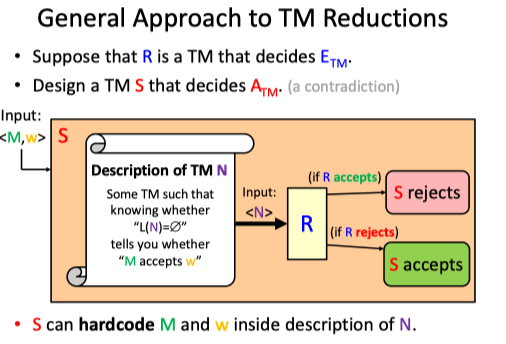
\includegraphics[scale=0.5]{general_approach_to_tm_reductions}

\underline{Reductions Tutorial Q4B}

Let $E_{TM} = \set{\encoding{M}: M \text{ is a TM s.t. } L(M) = \emptyset}$. Prove $E_{TM}$ is undecidable. Prove $\overline{E_{TM}}$ is recognizable. Is $E_{TM}$ recognizable?

Let $R$ be a TM that decides $E_{TM}$. Below is a TM $S$ that decides $A_{TM}$.

$S = $ on input $x$:

\begin{itemize}
    \item If $x$ not of form $\encoding{M, w}$, where $M$ is a TM, and $w \in \Sigma^*$, \emph{reject}.
    \item Construct $N$ = on input $y$:
    \begin{itemize}
        \item Run $M$ on $w$
        \item If $M$ rejects, \emph{reject}.
        \item Otherwise \emph{accept}.
    \end{itemize}
    \item Run $R$ on $\encoding{N}$.
    \item \emph{Reject} if $R$ accepts; otherwise \emph{accept}.
\end{itemize}

$S$ is a valid TM that decides $A_{TM}$ because:

\begin{itemize}
    \item when $M$ accepts $w$, $L(N) = \Sigma^*$, so $R$ rejects $\encoding{N}$, and thus, $S$ accepts.
    \item when $M$ rejects/runs forever on $w$, $L(N) = \emptyset$, so $R$ accepts $\encoding{N}$, and thus, $S$ rejects.
\end{itemize}

$A_{TM}$ is undecidable $\Rightarrow$ contradiction $\Rightarrow E_{TM}$ is undecidable.

$\overline{E_{TM}}= \set{\encoding{M}: M \text{ is a TM s.t. } L(M) \neq \emptyset} \\ \cup \set{x: x \text{ is not a valid encoding of a TM}}$. TM $U$ recognizes $\overline{E_{TM}}$.

$U$ = on input $x$:

\begin{itemize}
    \item If $x$ not of form of $\encoding{M}$, where $M$ is a TM, \emph{accept}.
    \item Nondeterministically choose a string $w \in \Sigma^*$, run $M$ on $w$.
    \item \emph{Accept} if $M$ accepts; otherwise \emph{reject}.
\end{itemize}

$U$ recognizes $\overline{E_{TM}}$ because:

\begin{itemize}
    \item when $x$ not of form $\encoding{M}$, $U$ accepts
    \item when $x = \encoding{M} \in \overline{E_{TM}}, L(M) \neq \emptyset$ which guesses a string $w \in L(M)$, and thus $U$ accepts in that branch.
    \item when $x = \encoding{M} \notin \overline{E_{TM}}, L(M) = \emptyset$, there is not string $w \in \Sigma^*$ which $M$ accepts, so the computation tree of $U$ does not have a branch that terminates in an acceptable state, and thus, $U$ rejects.
\end{itemize}

$\overline{E_{TM}}$ is recognizable and $E_{TM}$ is undecidable $\Rightarrow E_{EM}$ is not recognizable.

\section{Time Complexity}

\subsection{Time Complexity Classes}

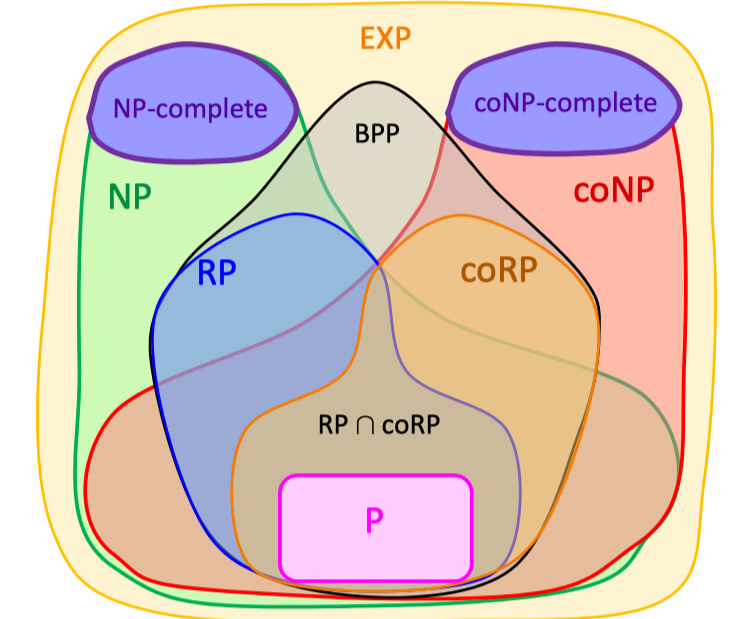
\includegraphics[scale=0.3]{time_complexity}

\begin{itemize}
    \item P is the class of languages that are decidable in polytime on a deterministic single-tape Turing machine. P $= \bigcup\limits_{k} TIME(n^k)$.
    \item NP is the class of languages $L$ for which one can efficiently verify membership in $L$. NP $= \bigcup\limits_{k} NTIME(n^k)$
    \item A language $B$ is NP-complete if:
    \begin{itemize}
        \item $B \in$ NP
        \item every $A \in$ NP is polytime reducible to $B$
    \end{itemize}
    \item coNP is a class of languages $L$ for which one can efficiently verify non-membership in $L$.
    \item $L \in$ RP if there is a PTM that, on input $x$, runs in time $poly(x)$, and has behavior:
    \begin{itemize}
        \item $x \in L$ if $Pr[\text{reaching accept}] \geq \frac{1}{2}$
        \item $x \notin L$ if $Pr[\text{reaching reject}] = 1$
    \end{itemize}
    \item $L \in$ coRP if there is a PTM that, on input $x$, runs in time $poly(x)$, and has behavior:
    \begin{itemize}
        \item $x \in L$ if $Pr[\text{reaching accept}] = 1$
        \item $x \notin L$ if $Pr[\text{reaching reject}] \geq \frac{1}{2}$
    \end{itemize}
    \item $L \in$ BPP if there is a PTM that, on input $x$, runs in time $poly(x)$, and has behavior:
    \begin{itemize}
        \item $x \in L$ if $Pr[\text{reaching accept}] \geq \frac{2}{3}$
        \item $x \notin L$ if $Pr[\text{reaching reject}] \geq \frac{2}{3}$
    \end{itemize}
    \item EXP $= \bigcup\limits_{k} TIME(2^{n^k})$.
\end{itemize}

\subsection{NP, coNP, RP, BPP}

\underline{NP is closed under union}:

Let $L_1, L_2 \in$ NP; $L_3 = L_1 \cup L_2$. $v_1$ and $v_2$ are verifiers for $L_1$ and $L_2$. $v_3 = v_1 \vee v_2$. $v_3$ is polytime $\Rightarrow L_3 \in$ NP.

% TODO: NP is closed under concatenation, complement, etc.

\underline{coNP is closed under union}:

Let $L_1, L_2 \in$ coNP; $L_3 = L_1 \cup L_2$. NTM's $M_1$ and $M_2$ that decide $\overline{L_1}$ and $\overline{L_2}$ in polytime. Construct $M_3$ that decides $\overline{L_1 \cup L_2} = \overline{L_1} \cap \overline{L_2}$ in polytime. Run $M_1$ and $M_2$. Accept if both accept, rejects otherwise.

\underline{coNP is closed under intersection}:

$\ldots \overline{L_1 \cap L_2} = \overline{L_1} \cup \overline{L_2} \ldots$. Run $M_1$ and $M_2$. Accept if either of them accepts, reject if both reject.

\underline{$L$ is NP-complete iff its complement is coNP-complete}

Suppose $L$ is NP-complete. Then $\overline{L}$ is in coNP because $L$ is in NP. Suppose $A$ is coNP, we want $A \leq_P \overline{L}$. Observe that $\overline{A}$ is in NP, and so $\overline{A} \leq_P L$ ($L$ is in NP-hard), but this is equivalent to saying $A \leq_P \overline{L}$ as desired. The other direction is similar.

\underline{if a coNP-complete problem in NP, then coNP = NP}

Suppose $A$ is coNP-complete and $A$ is in NP. Let $L$ be in coNP. Then $\overline{L}$ in NP. Because $\overline{A}$ is in NP-complete, $\overline{L} \leq_P \overline{A}$, which is equivalent to $L \leq_P A$. But since $A$ is in NP, then $L$ is also in NP. Let $L$ be in NP. Then $L \leq_P \overline{A}$ because $\overline{A}$ is NP-complete. Equivalently, $\overline{L} \leq A$. Because $A$ is in NP, then $\overline{L}$ is in NP, meaning $L$ is in coNP.

\underline{RP $\subset$ NP}

Convert a PTM into NTM by changing all probabilistic choices into non-deterministic choices. Let $L \in$ RP and $M$ be a PTM. After conversion, NTM correctly accepts/rejects $w \in L$ because:

\begin{itemize}
    \item $w \notin L$, PTM rejects $w$ with probability = 1, so does NTM.
    \item $w \in L$, PTM accepts $w$ with probability $\geq \frac{1}{2}$, so there is a computational path for NTM, which terminates in an accepting state.
\end{itemize}

\underline{RP and BPP are closed under union and intersection}

Let $L_1, L_2 \in$ RP, and two PTMs $M_1$, $M_2$.

$L_1 \cup L_2 \in$ RP. Run $M_1$ and $M_2$ independently on input $x$. Accept if either one of them accepts.

\begin{itemize}
    \item $x \in L_1 \setminus L_2$ or $x \in L_1 \setminus L_2$: $Pr[accept] \geq \frac{1}{2}$ of $M_1$ or $M_2$.
    \item $x \in L_1 \cap L_2$: $Pr[accept] \geq \frac{1}{2}$ of $M_1$ or $M_2$.
    \item $x \notin L_1$ or $x \notin L_1$: $Pr[reject] = 1$ of $M_1$ or $M_2$.
\end{itemize}

$L_1 \cap L_2 \in$ RP. Run $M_1$ and $M_2$ independently on input $x$. Accept if both of them accept.

\begin{itemize}
    \item One time: $Pr[accept] \geq \frac{1}{4}$.
    \item Three times: at least one trial where both accept $Pr[accept] = 1 - (1-\frac{1}{4})^3 \approx 0.58 \geq \frac{1}{2}$
\end{itemize}

BPP can be proven closed under union and intersection in a similar way.

\underline{RP $\subset$ BPP}

Let $L \in$ RP and PTM $M$.

$M'$ = on input $x$:

\begin{itemize}
    \item Run $M$ on $x$ twice.
    \item \emph{Accept} when one of the trials where $M$ accepts $x$.
\end{itemize}

Probabilities:

\begin{itemize}
    \item When $x \in L$, $Pr[reject] \leq \frac{1}{4}$.
    \item When $x \in L$, $Pr[accept] \geq \frac{3}{4}$.
    \item When $x \notin L$, $Pr[reject] = 1$.
\end{itemize}

\underline{BPP = coBPP}

Swap accepting and rejecting states.

\subsection{$3SAT$ Related Reductions}

\underline{$DOUBLESAT$}

$3SAT \leq DOUBLE-SAT$ by adding an extra Boolean variable to the $3SAT$ instance, so the 3CNF is satisfiable iff $DOUBLE-SAT$ has at least 2 satisfying assignments.

\underline{$CNF_3$}

Show $3SAT \leq_P CNF_3$.

Given a 3CNF formula $\phi$. For each variable $x$ give different names $x_1, \ldots, x_k$. Then we define $\phi_x = (x_1 \vee \neg x_2) \wedge (x_2 \vee \neg x_3) \wedge \ldots \wedge (x_k \vee \neg x_1)$. $a_1 = \ldots = a_k$ to satisfy $\phi_x$. $\varphi = \bigwedge_x \phi_x$.

\underline{$SUBSETSUM$}

$n$ variables $x_i$ and $m$ clauses $c_j$. For each variable $x_i$ construct numbers $t_i$ and $f_i$ of $n + m$ digits:

\begin{itemize}
    \item $i$-th digit of $t_i$ \& $f_i = 1$
    \item For $n + 1 \leq j \leq n + m$, $j$-th digit of $t_i = 1$ if $x_i$ is in clause $c_{j-n}$
    \item For $n + 1 \leq j \leq n + m$, $j$-th digit of $f_i = 1$ if $\overline{x_i}$ is in clause $c_{j-n}$
\end{itemize}

For each clause $c_j$, construct numbers $x_i$ \& $y_i$ of $n + m$ digits:

\begin{itemize}
    \item $n+j$-th digit of $x_j \& y_j = 1$
    \item Other $x_j \& y_j = 0$
\end{itemize}

Finally, construct a sum number $s$ of $n + m$ digits:

\begin{itemize}
    \item For $1 \leq j \leq n$, the $j$-th digit of $s = 1$.
    \item For $n + 1 \leq j \leq n + m$, the $j$-th digit of $s = 3$
\end{itemize}

\underline{$A_{TM}$}

$M$ = given a Boolean formula $w$, try all possible assignments and accept if any assignment satisfies $w$. Given a formula $\phi$, define $f(\phi) = \encoding{M, w}$. $f(\phi) \in A_{TM} \Rightarrow \phi \in 3SAT$.

\underline{$HALT_{TM}$}

$M$ = given a Boolean formula $w$, try all possible assignments. It runs forever, if a satisfiable assignment is not found. It only halts iff the $3SAT$ instance is satisfiable.

Output $\encoding{M, w}$.

\subsection{Graph Related Reductions}

\underline{$HALFCLIQUE$}

$G$ = graph with a clique of $k$ nodes. Construct graph $H$:

Case 1: $k \geq \frac{n}{2}$. $H$ = $G$ with $l$ isolated new nodes ($k = \ceil{\frac{n + l}{2}}$).

Case 2: $k \leq \frac{n}{2}$. $H$ = $G$ with $l$ new nodes, each of which is connected to every other node.

\underline{$DOMSET$}

Show $VC \leq_P DOMSET$

$G$ is a graph with a vertex cover of size $k$. Construct $G'$:

\begin{itemize}
    \item $G' = G$
    \item for each edge $(u, v)$ in $G$, add a new vertex $w_{uv}$ and new edges $\set{u, w_{uv}}$ and $\set{v, w_{uv}}$
    \item Let $I$ = \# isolated vertices and set $k' = k + n_I$
\end{itemize}

Output $\encoding{G', k'}$ for $DOMSET$.

\underline{$HITTING$}

Show $VC \leq_P HITTING$

$G$ is a graph with a vertex cover of size $k$. Let $\mathcal{U} =$ all vertices in $G$. For each edge $(u, v)$, $S_i = \set{u, v}$

\underline{$SETCOVER$}

Show $VC \leq_P SETCOVER$.

$G$ is a graph with a vertex cover of size $k$. Let $\mathcal{U} =$ all vertices in $G$. $S_i$ = set of edges incident to vertex $v_i$. $k$ is still the same.

\underline{$TSP$}

Show $HAMPATH \leq_P TSP$.

$\encoding{G} \in HAMPATH$. Construct $G'$:

\begin{itemize}
    \item $G' = G$
    \item $k = \abs{V}$
\end{itemize}

Output $\encoding{G', k}$ for $TSP$.

\subsection{Time Hierarchy Theorem}

For any time-constructable function $t: \mathcal{N} \rightarrow \mathcal{N}$, a language $A$ exists that is is decidable in $O(t(n))$ time but not decidable in $o(\frac{t(n)}{\log{t(n)}})$.

\textbf{Examples}:

\underline{P $\subseteq TIME(n^5)$?}

False. By THT, there exists $L \in TIME(n^{20}) \setminus TIME(n^5)$. Clearly $L \in$ P (since $TIME(n^{20}) \subseteq$ P). Thus, $L \in$ P, but $| \notin TIME(n^5)$.

\underline{E = $\bigcup_{c > 0} TIME(2^{cn})$ = EXP?}

False. By THT, there exists $L \in TIME(2^{4n^2}) \setminus TIME(2^{n^2})$. Clearly, $L \in$ EXP. Since $L \notin TIME(2^{n^2})$, the following claim implies $L \notin$ E, from which we conclude that E $\neq$ EXP. Claim: $E \subset TIME(2^{n^2})$. Proof: For $A \in $ E, there is a TM $M$ and constants $c, C, n_0 >0$ and its runtime is at most $C2^{cn} \; \forall n \geq n_0$. Note $C2^{cn} \leq C2^{n^2} \; \forall n \geq \max \set{c, n_0}$, so the runtime of $M$ is $O(2^{n^2})$. Thus, $A \in TIME(2^{n^2})$.

\section{Communication Complexity}

\subsection{Trivial Protocol}

\begin{itemize}
    \item Alice sends $x$ to Bob ($\lg(x)$).
    \item Bob computes $z$: $f(x, y)$.
    \item Bob sends $z$ to Alice ($\lg(z)$).
\end{itemize}

$D(f) \leq \lg(x) + \lg(z)$.

\subsection{Monochromatic Partition}

\begin{itemize}
    \item $C^{partition} (f) = \min \set{\abs{R}: R \text{ is a f-monochromatic partition}} \leq $ \# leaves of $T$
    \item For any protocol tree $T$, $\set{R_v: v \text{ is a leaf of } T}$ is an f-monochromatic partition.
    \item $D(f) \geq \ceil{\lg(C^{partition} (f))}$
\end{itemize}

\subsection{Fooling Sets}

Let $f: X \times Y \rightarrow Z$. A set $S$ is a fooling set for $f$ if :

\begin{itemize}
    \item All $(x, y) \in S$ have the same value $f(x, y) = z$.
    \item For all distinct $(x, y) \in S$ and $(x', y') \in S$, either $f(x', y) \neq z$ or $f(x, y') \neq z$.
\end{itemize}

$D(f) \geq \ceil{\log(\abs{S} + 1)}$

Examples:

\begin{itemize}
    \item $D(EQ_n) \geq n + 1$
    \item $D(GEQ_n) \geq n + 1$
    \item $D(DISJ_n) \geq n + 1$
\end{itemize}

\end{multicols*}

\end{document}
